\documentclass[12pt,a4paper]{article}
\usepackage[utf8]{inputenc}
\usepackage[spanish]{babel}
\usepackage{amsmath}
\usepackage{amsfonts}
\usepackage{amssymb}
\usepackage{graphicx}
\usepackage[left=17.3mm,right=17.3mm,top=19mm,bottom=25.4mm]{geometry}
\author{Jose Antonio Andrade Vieyra}
\title{Radio Digital.}
\usepackage{pdfpages}
\usepackage{enumerate}
\usepackage{parskip}
\usepackage{multicol}   
\usepackage{caption}
\captionsetup{font=scriptsize,labelfont=scriptsize}
\usepackage{listings}
\usepackage{color}
\setlength{\parskip}{6pt}
\definecolor{migris}{rgb}{0.5,0.5,0.5}
\definecolor{gray97}{gray}{.97}

\usepackage{tocloft}

\renewcommand{\cftfigfont}{Figura }
\renewcommand{\cfttabfont}{Tabla }

\lstset{ 
  captionpos=b,                    % Establece la posición de la leyenda del cuadro de código
  frame=single,	                   % Añade un marco al código
  language= Scilab,                 % El lenguaje del código
  numbers=left,                    % Posición de los números de línea (none, left, right).
  numbersep=5pt,                   % Distancia de los números de línea al código
  numberstyle=\small\color{migris}, % Estilo para los números de línea
  backgroundcolor=\color{white},   %color de font
  keywordstyle=\color{blue},       % estilo de las palabras clave
  commentstyle=\color{green},
  rulecolor=\color{black},         % Si no se activa, el color del marco puede cambiar en los saltos de línea entre textos que sea de otro color, por ejemplo, los comentarios, que están en verde en este ejemplo
  stepnumber=1,                    % Muestra solamente los números de línea que corresponden a cada salto. En este caso: 1,3,5,...
  tabsize=4,                   % Establece el salto de las tabulaciones a 2 espacios
  basicstyle=\scriptsize\ttfamily,  
}
\renewcommand{\lstlistingname}{Código}         %  Listings


\begin{document}

%Inicio portada--------------------------------------------------------------------------------
\begin{titlepage}
\begin{figure}[h!]
\centering

\includegraphics[scale=1]{LOGO.png}
\end{figure}
\hspace{1.3cm}\rule{14.5cm}{3pt} \hspace{-16.5cm}
\rotatebox{270}{\rule{20cm}{3pt}}\hspace{0.43cm} \rotatebox{270}{\rule{18.5cm}{3pt}}\hspace{0.43cm} \rotatebox{270}{\rule{16.98 cm}{3pt}}\vspace{-19cm}
\begin{center}
\hspace{1.3cm} {\bf{\fontsize{20pt}{20pt} \selectfont INSTITUTO TECNOLÓGICO DE}}\\[0.5cm]
\hspace{1.3cm} {\bf{\fontsize{20pt}{20pt} \selectfont MORELIA}}\\[2cm]
\hspace{1.3cm} {\fontsize{20pt}{20pt} \selectfont Control I.}\\[1cm]
\hspace{1.3cm} {\fontsize{20pt}{20pt} \selectfont Ingeniería Electrónica}\\[1cm]
\hspace{1.3cm} {\bf{\fontsize{18pt}{18pt} \selectfont Práctica \#1:}}\\[0.5cm]
\hspace{1.3cm} {\bf{\fontsize{18pt}{18pt} \selectfont Analysis of a first order system.}}\\[1.5cm]
\hspace{1.3cm} {\fontsize{16pt}{16pt} \selectfont Presentan:}\\[0.8cm]
\hspace{1.3cm} {\bf{\fontsize{14pt}{14pt} \selectfont José Antonio Andrade Vieyra No. Control:14121110}}\\[0.5cm]
\hspace{1.3cm} {\bf{\fontsize{14pt}{14pt} \selectfont Gerardo García Torres No. Control: 14121118}}\\[1cm]
\hspace{1.3cm} {\fontsize{16pt}{16pt} \selectfont Asesor:}\\[0.5cm]
\hspace{1.3cm} {\bf{\fontsize{14pt}{14pt} \selectfont Gerardo Marx Chávez Campos}}
\end{center}   
\vspace{1.8cm}\hspace{1.3cm}\raggedleft {\fontsize{11pt}{11pt} \selectfont Morelia, Michoacán 27 de Octubre del 2017}
\end{titlepage}
%Final portada---------------------------------------------------------------------------------

%Introducción-------------------------------------------------------------------------------
\newpage
\section{Introducción.}
Una función de transferencia es un modelo matemático que a través de un cociente relaciona la respuesta de un sistema (modelada) con una señal de entrada o excitación (también modelada) en palabras más simples, quiere decir que este modelo matemático nos relaciona la entrada con la salida de un sistema.\\
	En la teoría de control, a menudo se usan las funciones de transferencia para caracterizar las relaciones de entrada y salida de componentes o de sistemas que se describen mediante ecuaciones diferenciales lineales e invariantes en el tiempo.\\
	La definición formal para sistemas invariantes en el tiempo o sistemas lineales (LTI): \\
	\\\textit{Se define como el cociente entre la transformada de Laplace de la salida y la transformada de Laplace de la entrada, bajo la suposición de que las condiciones iniciales son nulas.}
	
	\subsection{Descripción Matemática}
	Uno de los primeros matemáticos en describir estos modelos fue Laplace de manera que tiene una interpretación inmediata en la frecuencia $s = j\omega$, haciendo uso de su transformada matemática, que por definición una función de transferencia se puede determinar de la siguiente forma:
	
	\begin{equation*}
		H(s) = \frac{Y(s)}{X(s)}
	\end{equation*}
	
	Donde:\\
	$H(S)$ es la función de transferencia, que también puede denotarse por $G(S)$.\\
	$Y(S)$ es la respuesta o salida del sistema.\\
	$X(S)$ es la señal de entrada.\\
	\\
	La función de transferencia también puede considerarse como la respuesta de un sistema inicialmente inerte a un impulso como señal de entrada:
	
	\begin{equation*}
		H(S) = \mathcal{L}  \{h(t)\} = \int_{0}^{\infty} e^{-St} h(t) dt
	\end{equation*}
	
	De manera que podemos conocer la respuesta del sistema de la siguiente forma:
	
	\begin{equation*}
		Y(S) = X(S)H(S)
	\end{equation*}
	
	y la respuesta en el domino del tiempo seria:
	
	\begin{equation*}
		y(t) = \mathcal{L}^{-1} [Y(S)]
	\end{equation*}
	
	Cualquier sistema físico (mecánico, eléctrico, etc.) se puede traducir a una serie de valores matemáticos a través de los cuales se conoce el comportamiento de estos sistemas frente a valores concretos.\\
	\\
	Podemos generalizar las funciones de transferencia para los sistemas que estemos analizando, recordando que las funciones de transferencia en su mayoría se usan para caracterizar sistemas que depende de ecuaciones diferenciales, la función de transferencia para un sistema de primer orden seria:
	
	\begin{equation*}
		H(S) = \frac{bS + c}{a + dS}
	\end{equation*}
%------------------------------------------------------------------------------------------

%Desarrollo-------------------------------------------------------------------------------
\section{Metodología.}
Para la primera parte de la práctica se entendió el procedimiento para obtener la función de transferencia, así como obtener la respuesta de escalón unitario para la respuesta al sistema. Primero se tiene que considerar un sistema con una entrada $u(t)$ y una salida $y(t)$, con esto la función de transferencia estara dada por la Ecuación \ref{Ecuacion1}.
\begin{equation}
\centering
H(s) = \dfrac{Y(s)}{U(s)}
\label{Ecuacion1}
\end{equation}
Se puede observar que la Ecuación \ref{Ecuacion1} esta en terminos de $s$, es decir que se aplica la transformada de Laplace a la función de tiempo. Con esto es posible calcular la salida con cero condiciones iniciales considerando una entrada de escalon unitadrio como se observa en la Ecuación \ref{Ecuacion2} y \ref{Ecuacion3}.
\begin{equation}
Y(s) = X(s)H(s)
\label{Ecuacion2}
\end{equation}
\begin{equation}
Y(s) = \dfrac{1}{s}H(s)
\label{Ecuacion3}
\end{equation}
Ahora considerando una función de transferencia de primer orden generica donde solo se modificaran los coeficientes con números reales:
\begin{equation}
\centering
H(s) = \dfrac{bs + c}{ds + a}
\label{Ecuacion5}
\end{equation}
Con lo anterior, se obtiene la Ecuación \ref{Ecuacion4} que seria nuestra respuesta de escalón unitario generica dada nuestra función de transferencia $H(s)$.
\begin{equation}
\centering
Y(s) = \dfrac{1}{s}\dfrac{bs + c}{ds + a}
\label{Ecuacion4}
\end{equation}
Después como se ha visto en clase se aplica fracciones parciales para poder, posteriormente, aplicar transformada inversa de laplace a cada termino.
\begin{center}
$Y(s) = \dfrac{A}{s} + \dfrac{B}{ds + a}$
\end{center}
Para encontrar los valores de A y B se hizo lo siguiente:
\begin{center}
$A: \dfrac{bs+c}{ds + a}$ Donde $s = 0$ entonces: $\mathbf{A = \dfrac{c}{a}}$\\[12pt]
$B: \dfrac{bs+c}{ds + a}$ Donde $s = \dfrac{-a}{d}$ entonces: $\mathbf{B = \dfrac{ba-cd}{a}}$
\end{center}
Con esto $Y(s)$ queda:
\begin{center}
$Y(s) = \dfrac{\dfrac{c}{a}}{s} + \dfrac{\dfrac{ba - cd}{ad}}{s + \dfrac{a}{d}}$
\end{center}
Aplicando la transformado inversa de laplace nos quedaria la Ecuación \ref{Ecuacion6}:
\begin{equation}
\centering
y(t) = \frac{c}{a} + {\frac{ba-cd}{ad}}e^{(-a/dt)}
\label{Ecuacion6}
\end{equation}
Entonces ahora solo dando los coeficientes podemos obtener nuestra respuesta de escalón unitario con el programa hecho en Scilab. Posteriormente, se analizó el sistema hidráulico de la Figura \ref{Figura1}.\\
\begin{figure}[h!]
\centering
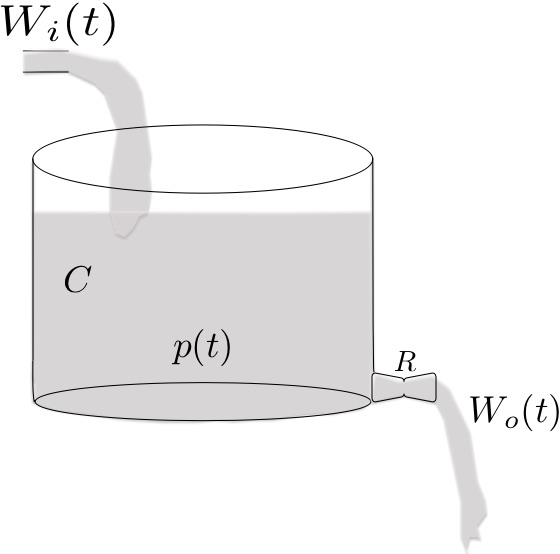
\includegraphics[scale=0.5]{Tank.jpg}
\caption{Sistema hidráulico a analizar.}
\label{Figura1}
\end{figure}\\
Como se puede observar el tanque tiene diferentes variables y constantes, la ecuación de balance de este sistema se muestra en la Ecuación \ref{Ecuacion7}.
\begin{equation}
\centering
W_{in}(t) = W_{o}(t) + A\dfrac{dh(t)}{dt}
\label{Ecuacion7}
\end{equation} 
Donde:
\begin{enumerate}[$\cdot$]
\item $W_{in}(t)$ es la cantidad de agua de entrada en $\frac{m^{3}}{s}$
\item $W_{o}(t)$ es la cantidad de agua de salida en $\frac{m^{3}}{s}$
\item $A$ es el area del tanque en $m^2$
\item $h(t)$ es la altura del tanque que esta cambiando constantemente.
\end{enumerate}
$W_{o}(t)$ esta siendo determinado por la resistencia, altura de la llave y de la gravedad por lo que se puede reemplazar por:
\begin{center}
$W_{o}(t) = \dfrac{rgh(t)}{R}$
\end{center}
Viendo este sistema desde un punto de vista de circuito eléctrico, el area sería la capacitancia $Ce$ y el coeficiente de $\frac{rg}{R}$ sería el inverso de la resistencia eléctrica $Re$, por lo que nuestra Ecuación \ref{Ecuacion7} quedaría como la Ecuación \ref{Ecuacion8}.
\begin{equation}
\centering
W_{in}(t) = \dfrac{h(t)}{Re} + Ce\dfrac{dh(t)}{dt}
\label{Ecuacion8}
\end{equation}
Con esto podemos hacer una interpretación de la Ecuación anterior para obtener una igualdad en un circuito eléctrico, el circuito eléctrico resultante se muestra en la Figura \ref{Figura2}.\\
\begin{figure}[h!]
\centering
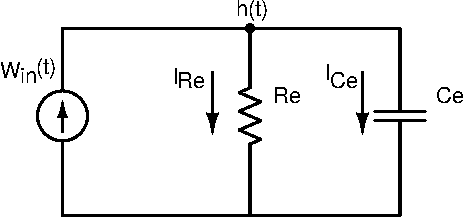
\includegraphics[scale=1]{Circuito.pdf}
\caption{Circuito eléctrico resultante de la Ecuación \ref{Ecuacion8}.}
\label{Figura2}
\end{figure}\\
Donde:
\begin{center}
$I_{Re}=\dfrac{h(t)}{Re}$\hspace{5cm}$I_{Ce}=Ce\dfrac{dh(t)}{dt}$
\end{center}
Con esto concluimos que $I_{Re}$ es la salida del sistema y $I_{Ce}$ es la constante que contiene la altura que se esta cambiando constantemente. Esto nos ayudara a entender más adelante los 3 casos que se piden.\\[12pt]
Ahora obtenemos la función de transferencia de primer orden de nuestro sistema hidráulico aplicando la transformada de Lapla a la Ecuación \ref{Ecuacion8}.
\begin{center}
$\mathcal{L}\left\lbrace W_{in}(t) = \dfrac{h(t)}{Re} + Ce\dfrac{dh(t)}{dt} \right\rbrace$\\[15pt]
$W_{in}(s) = \dfrac{h(s)}{Re} + Cesh(s)$
\end{center}
Despejando para obtener $\frac{h(s)}{W_{in}(s)}$ ya que es $h(t)$ el que nos interesa ya que esta en constante cambio.
\begin{equation}
\centering
\dfrac{h(s)}{W_{in}(s)} = \dfrac{Re}{1 + ReCes}
\label{Ecuacioncod}
\end{equation}
\begin{center}
$\dfrac{h(s)}{W_{in}(s)} = \dfrac{Re(\frac{1}{ReCe})}{(1 + ReCes)(\frac{1}{ReCe})}$\\[12pt]
$\dfrac{h(s)}{W_{in}(s)} = \dfrac{\frac{1}{Ce}}{s + \frac{1}{ReCe}}$
\end{center}
Entonces nuestra función de transferencia de primer orden se muestra en la Ecuación \ref{Ecuacion9}.
\begin{equation}
\centering
H(s) = \dfrac{\frac{1}{Ce}}{s + \frac{1}{ReCe}}
\label{Ecuacion9}
\end{equation}
Comparando con la Ecuación \ref{Ecuacion5} nuestros coeficientes serían:
\begin{center}
$a = \frac{1}{ReCe}$\hspace{3cm}$b = 0$\hspace{3cm}$c = \frac{1}{Ce}$\hspace{3cm}$d = 1$\end{center}
\newpage
%-----------------------------------------------------------------------------------------

%Resultados y discuciones-----------------------------------------------------------------
\section{Resultados y discusiones.}
El código proporcionado de Scilab para obtener la función de respuesta de escalon unitario se muestra en el Código 1 y el código hecho por nosotros para obtener dicha función se encuentra en el Código 2.
\begin{center}
\lstinputlisting[caption=Código proporcionado de Scilab.]{Primergradofuncion.sce}
\end{center}
\begin{center}
\lstinputlisting[caption=Código hecho por nosotros para obtener respuesta de escalón unitario.]{Obtenertransf.sce}
\end{center}
Se puede observar que en el Código 1 en la 13 tenemos la función de transferencia con constantes Tau y $K$, esta ecuación es la Ecuación \ref{Ecuacioncod} donde $K = Re$ y $Tau = ReCe$. El Código 2 es simple ademas esta comentado por lo que no se explicara su funcionamiento.\\[12pt]
En la Figura \ref{Figura3} y en la Figura \ref{Figura4} se muestra la comparacion de la obtención de resultados de los 2 códigos esto se muestra mediante gráficas donde $Re = 1$ y $Ce=1$, por lo que en el Código 1 $K = 1$ y $Tau = 1$ y en el Código 2 $a = 1$, $b = 0$, $c = 1$ y $d = 1$ y se puede observar que son parecidas por lo que el Código 2 funciona correctamente.
\begin{figure}[h!]
\begin{minipage}{8cm} 
\centering
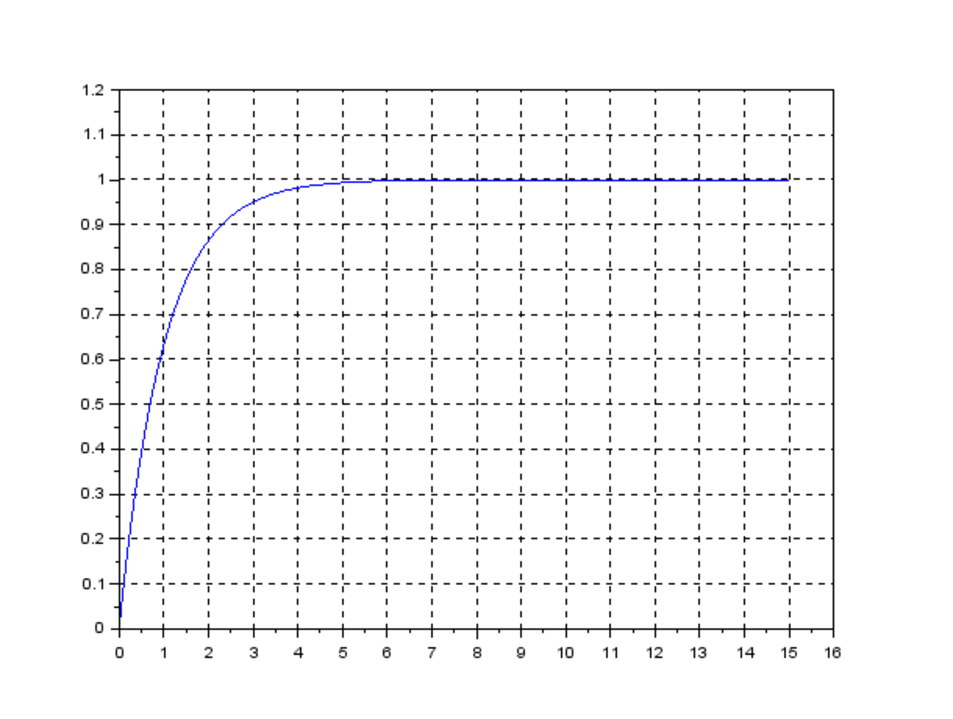
\includegraphics[scale=0.4]{Comparacion_profe.pdf}
\caption{Gráfica hecha con el Código 1 con $K = 1$ y $Tau = 1$.}
\label{Figura3}
\end{minipage}
\hspace{0.5cm}
\begin{minipage}{8cm}
\centering
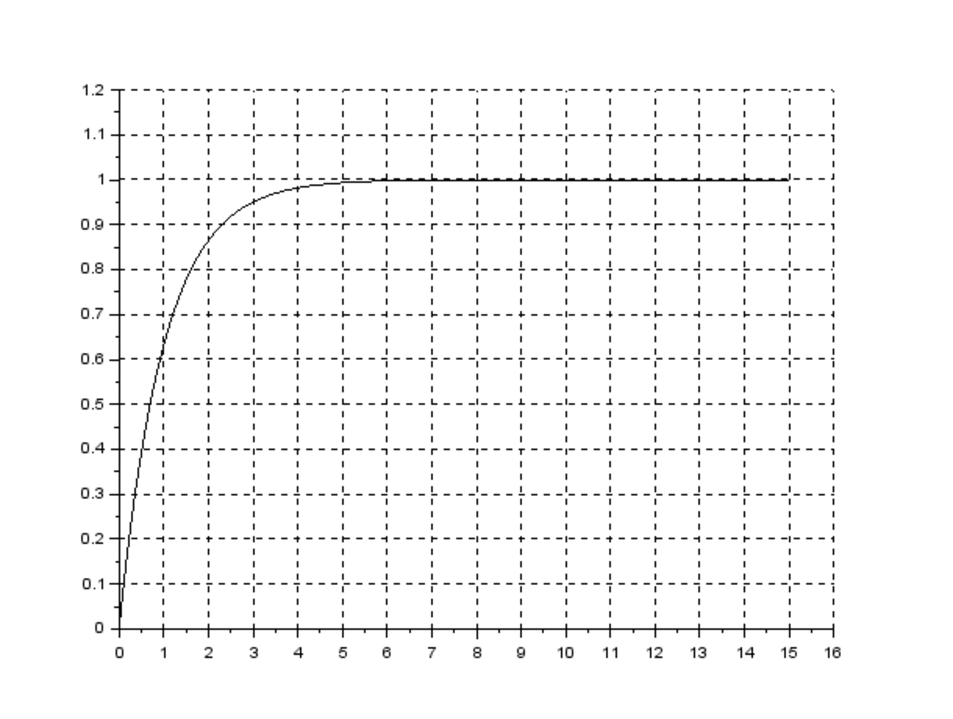
\includegraphics[scale=0.4]{Comparacion_yo.pdf}
\caption{Gráfica hecha con el Código 1 con $a = 1$, $b = 0$, $c = 1$ y $d = 1$.}
\label{Figura4}
\end{minipage}
\end{figure}\\
A continuación se desarrollan los resultados obtenidos de los 3 casos:
\begin{enumerate}[$\cdot$]
\item $W_{in}(t) = W_{o}(t)$
\item $W_{in}(t) > W_{o}(t)$
\item $W_{in}(t) < W_{o}(t)$
\end{enumerate}
\subsection{Caso: $\mathbf{W_{in}(t) = W_{o}(t)}$.}
Para este caso se tiene la Ecuación \ref{Ecuacion7}:
\begin{center}
$W_{in}(t) = W_{o}(t) + A\dfrac{dh(t)}{dt}$
\end{center}
Como $W_{in}(t) = W_{o}(t)$ el termino $A\frac{dh(t)}{dt}$ tiene que ser cero entonces se deduce lo siguiente:
\begin{center}
$A = 0$ \hspace{2cm} ó \hspace{2cm} $\dfrac{dh(t)}{dt} = 0$
\end{center}
Por lo que $h(t)$ no esta variando constantemente y se mantiene en un mismo nivel, esto suene coherente ya que para que sea la misma salida que la entrada solo tiene que haber un tubo entre los dos sin una resistencia o sin un contenedor. Entonces nos queda lo siguiente:
\begin{center}
$W_{in}(t) = \dfrac{h(t)}{Re}$\\[12pt]
$\mathcal{L}\left\lbrace W_{in}(t) = \dfrac{h(t)}{Re}\right\rbrace$\\[12pt]
$W_{in}(s) = \dfrac{h(s)}{Re}$\\[12pt]
$H(s) = Re$
\end{center}
Nuestra función de transferencia queda lineal dado el valor de $Re$. Por lo tanto nuestros coeficientes para meter a los códigos son los siguientes:
\begin{center}
$K = Re$\hspace{3cm}$Tau = 0$\hspace{3cm}$a= 1$\hspace{3cm}$b = 0$\hspace{3cm}$c = Re$\hspace{3cm}$d = 0$
\end{center} 
Dando el valor de $Re = 1$ entonces $H(s) = 1$ y $y(t) = 1$, se obtiene las siguientes dos Figura \ref{Figura5} donde se ve como actua la respuesta de escalón unitario.\\[12pt]
\begin{figure}[h!] 
\centering
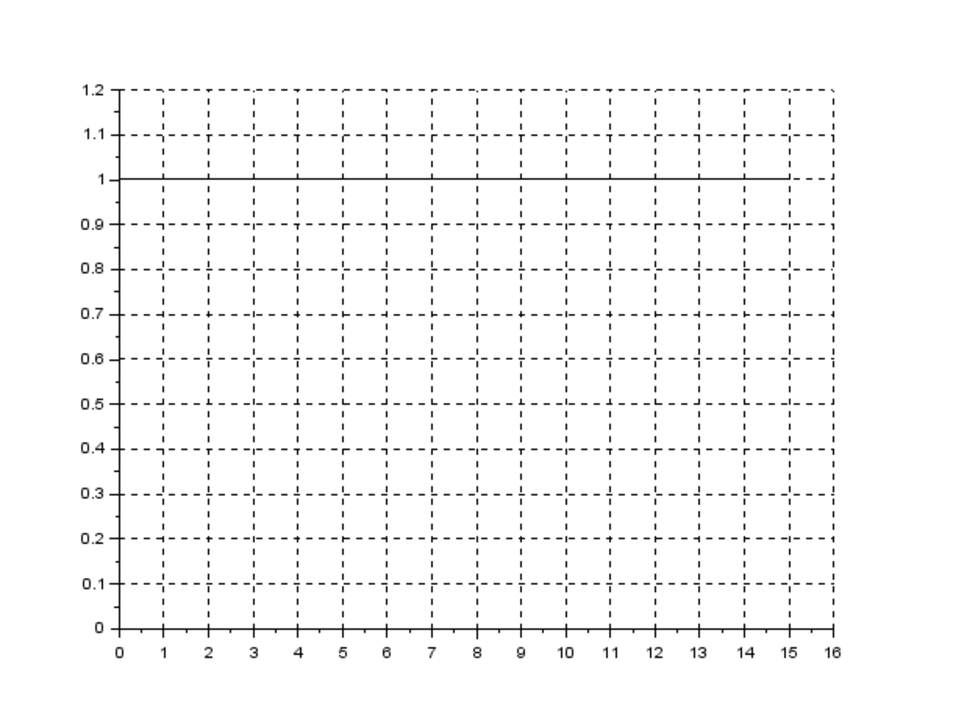
\includegraphics[scale=0.4]{WiIgualWo_yo.pdf}
\caption{Gráfica de respuesta de escalón unitario con $a = 1$, $b = 0$, $c = 1$ y $d = 0$.}
\label{Figura5}
\end{figure}\\
No se pudo hacer la gráfica con el Código 1 ya que Tau tendría que ser 0 no y no obtenia los valores para y(t). Efectivamente en la Figura \ref{Figura5} se observa que es lineal.
\subsection{Caso: $\mathbf{W_{in}(t) > W_{o}(t)}$.}
Para este caso se tiene la Ecuación \ref{Ecuacion7}:
\begin{center}
$W_{in}(t) = W_{o}(t) + A\dfrac{dh(t)}{dt}$
\end{center}
$W_{in}(t) > W_{o}(t)$, esto se puede entender mejor viendo el circuito de la Figura \ref{Figura2} ya que la corriente $I_{Re}$ tiene que ser menor que la otra esto indica lo sigueinte:
\begin{center}
$Ce > \dfrac{1}{Re}$
\end{center}
Por lo que $Ce$ tiene que ser mayor al inverso de la $Re$, esa seria nuestra condición principal,esto seria que la $Re$ tiene que ser muy grande para que no haya mucho corriente pasando por la resistencia y viendolo desde el punto hidráulico en la llave tiene que haber mucha resistencia para que no pase tanta agua y asi se cumpla la condición de este caso haciendo que el nivel de agua ascienda. Entonces nuestra función de transferencia sería la misma que la Ecuación \ref{Ecuacion9} solo cumpliendo la condición:
\begin{center}
$H(s) = \dfrac{\frac{1}{Ce}}{s + \frac{1}{ReCe}}$
\end{center}
Por lo tanto nuestros coeficientes para meter a los códigos son los siguientes:
\begin{center}
$K = Re$\hspace{3cm}$Tau = ReCe$\hspace{3cm}$a = \frac{1}{ReCe}$\hspace{3cm}$b = 0$\hspace{3cm}$c = \frac{1}{Ce}$\hspace{3cm}$d = 1$
\end{center} 
Dando el valor de $Re = 100$ y de $C=1$:
\begin{center}
$K = 100$\hspace{3cm}$Tau = 100$\hspace{3cm}$a = 0.01$\hspace{3cm}$b = 0$\hspace{3cm}$c = 1$\hspace{3cm}$d = 1$\\[12pt]
$H(s) = \dfrac{1}{s + 0.01}$\\[12pt]
$y(t) = 100 - 100e^{-0.01t}$\\[12pt]
\end{center} 
Se obtiene las siguientes dos Figura \ref{Figura6} y \ref{Figura7} donde se ve como actua la respuesta de escalón unitario.\\
\begin{figure}[h!]
\begin{minipage}{8cm} 
\centering
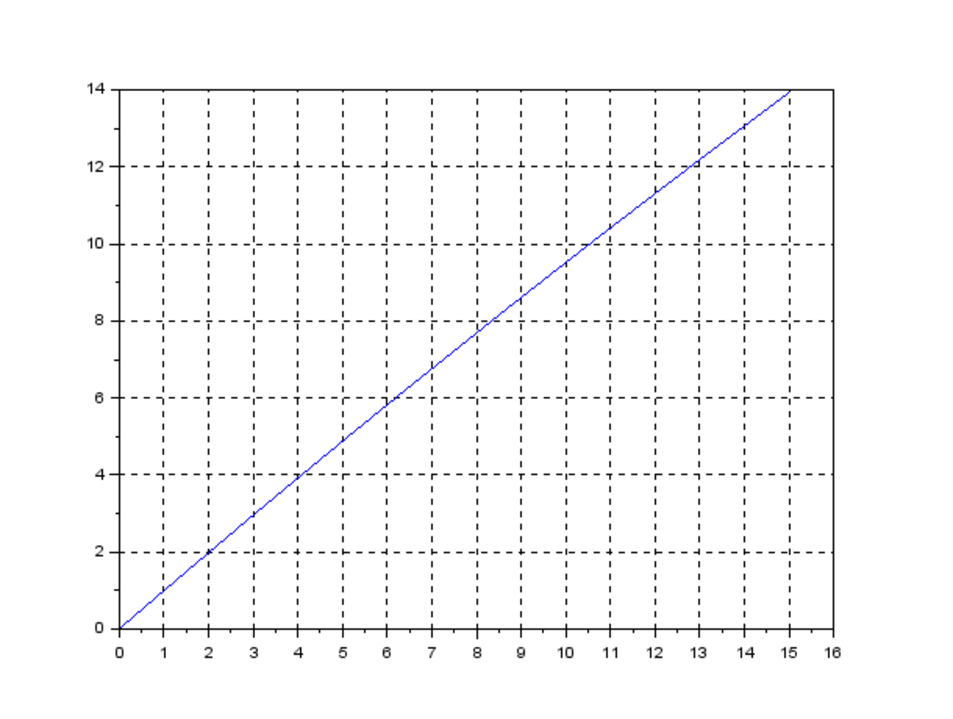
\includegraphics[scale=0.4]{WiMayorWo_profe.pdf}
\caption{Gráfica usando Código 1 con $Tau = 100$ y $K=100$.}
\label{Figura6}
\end{minipage}
\hspace{0.5cm}
\begin{minipage}{8cm}
\centering
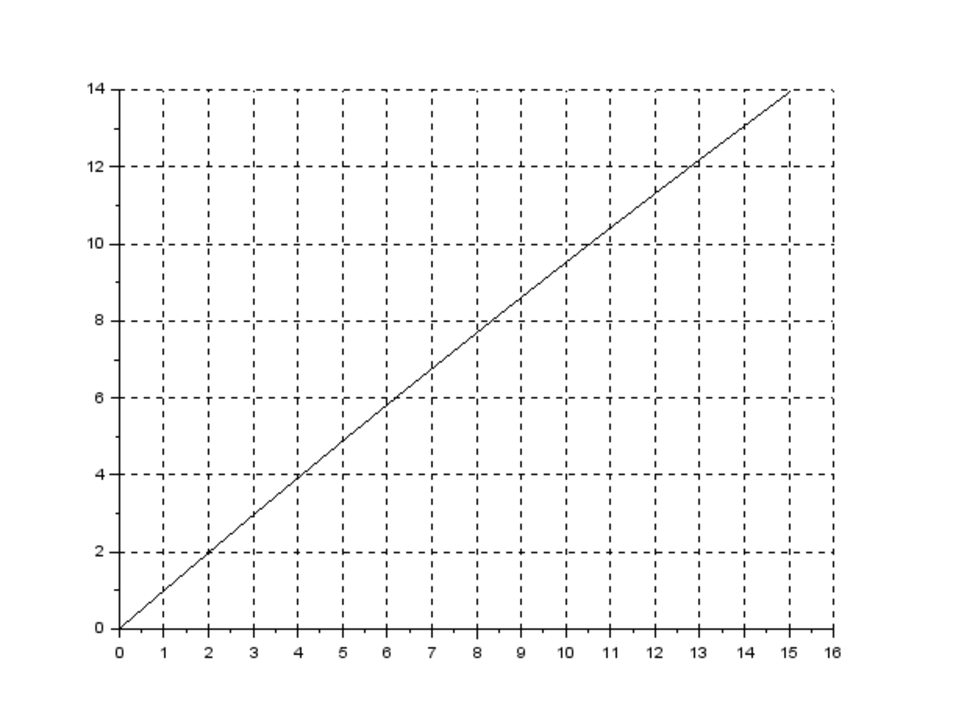
\includegraphics[scale=0.4]{WiMayorWo_yo.pdf}
\caption{Gráfica usando Código 2 con $a = 0.01$, $b = 0$, $c = 1$ y $d = 1$.}
\label{Figura7}
\end{minipage}
\end{figure}
\newpage
\subsection{Caso: $\mathbf{W_{in}(t) < W_{o}(t)}$.}
Para este caso se tiene la Ecuación \ref{Ecuacion7}:
\begin{center}
$W_{in}(t) = W_{o}(t) + A\dfrac{dh(t)}{dt}$
\end{center}
Proponiendo que $W_{in}(t) = 5$ y $W_{o}(t) = 10$ se obtiene lo siguiente:
\begin{center}
$5 = 10 + Ce\dfrac{dh(t)}{dt}$\\[12pt]
$\dfrac{5-10}{Ce} = \dfrac{dh(t)}{dt}$
$\dfrac{-5}{Ce} = \dfrac{dh(t)}{dt}$
\end{center}
Se puede observar que la derivada queda con un valor constante negativo, esto es la derivada de una linea recta con pendiente negativa, por lo que indica que el nivel de agua esta callendo y termina siendo este termino negativo. Nuestra función de transferencia queda así:
\begin{center}
$W_{in}(t) = W_{o}(t) + Ce\dfrac{dh(t)}{dt}$\\[12pt]
$\mathcal{L}\left\lbrace W_{in}(t) = W_{o}(t) + Ce\dfrac{dh(t)}{dt}\right\rbrace$\\[12pt]
$W_{in}(s) = \dfrac{h(s)}{Re} - sCeh(s)$\\[12pt]
$\dfrac{h(s)}{W_{in}(s)} = \dfrac{Re}{1-ReCes}$\\[12pt]
$H(s) = \dfrac{\frac{-1}{Ce}}{s-\frac{1}{ReCe}}$
\end{center}
Por lo tanto nuestros coeficientes para meter a los códigos son los siguientes:
\begin{center}
$K = Re$\hspace{3cm}$Tau = -ReCe$\hspace{3cm}$a = \frac{-1}{ReCe}$\hspace{3cm}$b = 0$\hspace{3cm}$c = \frac{-1}{Ce}$\hspace{3cm}$d = 1$
\end{center} 
Dando el valor de $Re = 10$ y de $C=1$:
\begin{center}
$K = 10$\hspace{3cm}$Tau = -10$\hspace{3cm}$a = -0.1$\hspace{3cm}$b = 0$\hspace{3cm}$c =-1$\hspace{3cm}$d = 1$\\[12pt]
$H(s) = \dfrac{-1}{s - 0.1}$\\[12pt]
$y(t) = 10 - 10e^{0.1t}$\\[12pt]
\end{center} 
Se obtiene las siguientes dos Figura \ref{Figura8} y \ref{Figura9} donde se ve como actua la respuesta de escalón unitario.\\[12pt]
Donde se puede observar que efectivamente hay una caída en la función, se penso, si el flujo de entrada es menor que el de la salida, de forma física el contenedor jamás tendra altura, pero si esto lo analizaramos con una condición inicial en donde decimos que el contenedor ya tenia agua con 1m de altura por ejemplo y le aplicamos el flujo de entrada menor al flujo de salida el tanque se va a comenzar a vaciar pero no de manera lineal, esto se debe a que aun se tine un flujo de entrada que no es lo suficiente para mantener o elevar la altura del agua pero si para que su vaciado no sea lienal.
\begin{figure}[h!]
\begin{minipage}{8cm} 
\centering
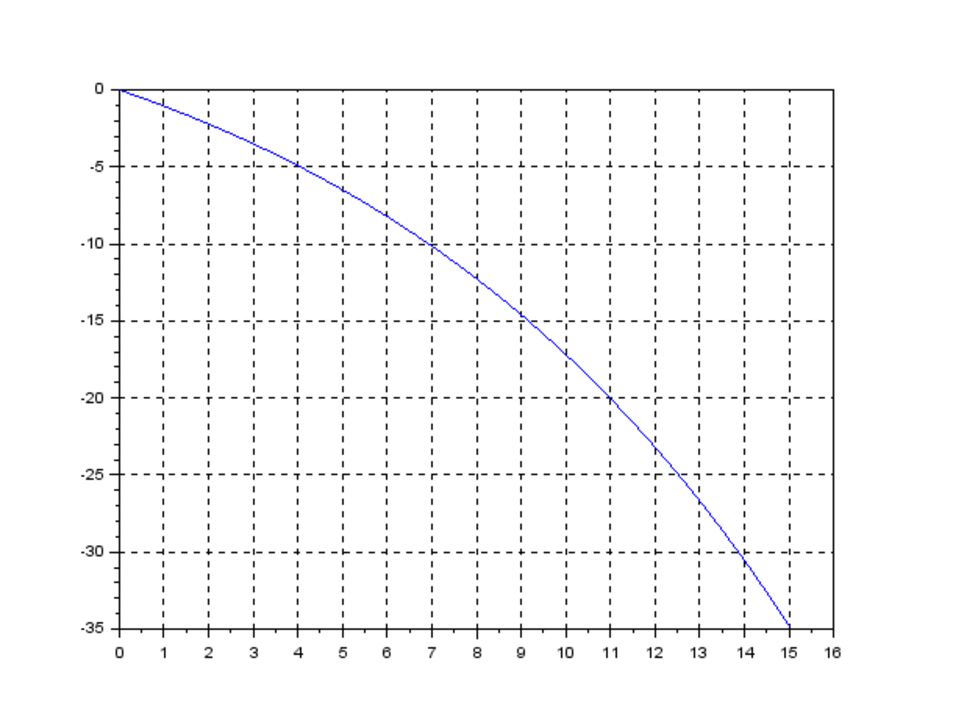
\includegraphics[scale=0.5]{WiMenorWo_profe.pdf}
\caption{Gŕafica hecha por el Código 1 con $Tau=-10$ y $K=10$.}
\label{Figura8}
\end{minipage}
\hspace{0.5cm}
\begin{minipage}{8cm}
\centering
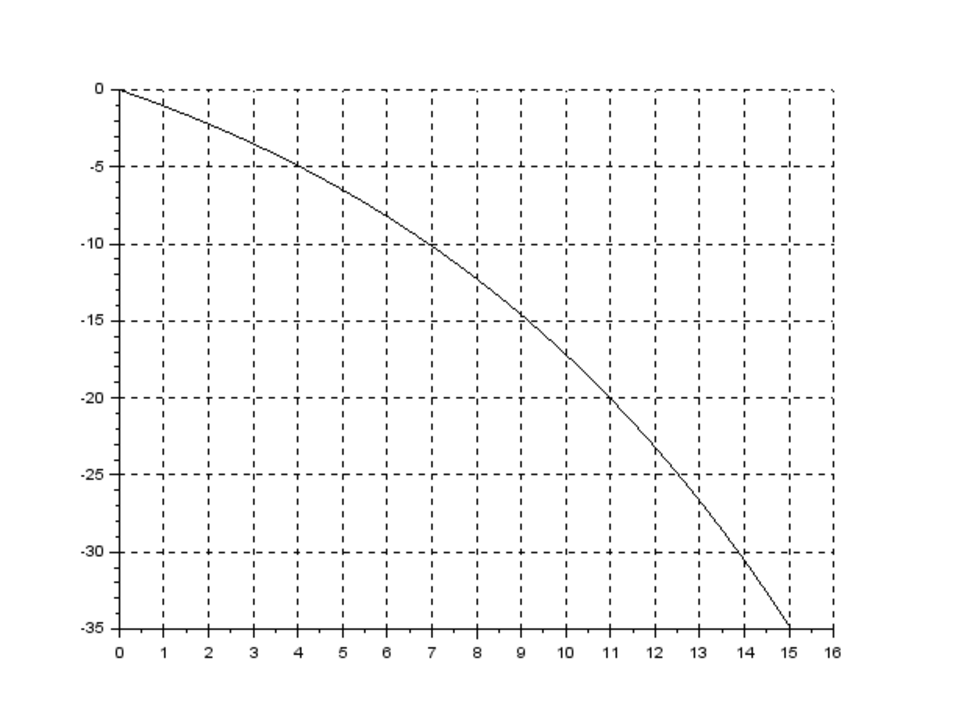
\includegraphics[scale=0.5]{WiMenorWo_yo.pdf}
\caption{Gráfica hecha por el Código 2 con $a = -0.1$, $b = 0$, $c =-1$ y $d = 1$.}
\label{Figura9}
\end{minipage}
\end{figure}\\
\newpage
%-----------------------------------------------------------------------------------------

%Conclusion-------------------------------------------------------------------------------
\section{Conclusión de Gerardo Garcia Torres.}
La función de transferencia nos permite conocer información del sistema que se está estudiando, en el caso de esta práctica por ejemplo, modelábamos un sistema hidráulico, haciendo uso de analogías lo transformamos en un modelo eléctrico el cual es conocido por lo que es más fácil interpretarlo, al realizar en el sistema 3 comparaciones diferentes podemos ver que gracias a la interpretación de la función de transferencia y la analogía eléctrica, podemos modificar el comportamiento del sistema sin necesidad de hacer pruebas experimentales. Al conocer en la analogía eléctrica su equivalencia con el modelo físico, podemos controlar la salida del sistema respecto la señal de entrada, también es importante tener la capacidad de visualizar lo que está sucediendo con el sistema, esto quiere decir que al no tener el sistema hidráulico de forma física y emplear la analogía eléctrica, los resultados matemáticos nos conducen a la respuesta, pero si no se tiene la visualización de lo que está sucediendo con el sistema y como esta respuesta seria en el sistema hidráulico, podemos llegar a cometer errores.
\section{Conclusión de Jose Antonio Andrade Vieyra.}
Con esta práctica se entendió como usar las ecuaciones para equilibrar un sistema, en este caso fue de un sistema hidráulico a parte de que se aprendió mejor como igualar este sistema a un circuito eléctrico para entender mejor su funcionamiento y así poder sacar conclusiones más facilmente ya que nosotros tenemos un mejor entendimiento en los circuitos eléctricos. Con esto también nos dimos cuenta que tan laborioso puede ser un circuito RC, ya que fue la igualdad al sistema y que tanto puede tener de importancia este circuito.\\[12pt]
Además en esta práctica se pudo observar los 3 casos para un sistema de paso de agua a un contenedor y despues a una salida, estos 3 casos fueron cuando no hay contenedor, cuando el agua en el contenedor asciende y cuando en el agua en el contender desciende. Principalmente tuvimos problemas para el 3er caso ya que fue dificil encontrar esta relación pero gracias a que se hizo paso a paso en la ecuación y dandole valores a la entrada y salida se dedujo que la derivada daba negativa por lo que esto indicaba que el nivel de agua caía. Ya con los otros 2 casos fue más sencillo ya que con ayuda del profesor en clase nos ayudo diciendo que lo vieramos desde el punto de vista eléctrico y así fue más sencillo. 
%-----------------------------------------------------------------------------------------

\end{document}
